
%%% Local Variables:
%%% mode: latex
%%% TeX-master: "www2019"
%%% End:

\section{Tracking in a rectangle-like area}
\label{sec:rectangle}
Currently, position tracking and trajectory tracking methods both use \sed as the distance metric to check data points and confirm the actual position of a moving object at time $t$ lives in a circle around the excepting position of the moving object at that time.
{However, as mentioned in Section~\ref{sec-intro}, there is a need of tracking a moving object in other areas, \ie a strip or rectangular area.}
Note that, though it is possible to track a moving object in a rectangular area, it is really hard to design such a shape without introducing a new distance metric other than the well-known metrics \sed and \ped, and at the same time develop an efficient algorithm for that.
Alternatively, this section defines a rectangle-like area that subtly makes use of \ped and \sed, and then develops such an effective and efficient trajectory tracking algorithm.
%, and (2) a circular or strip area is indeed a special case of a rectangle-like area.
%as in \cite{Lin:Dual}, 

\subsection{Building the rectangle-like areas}

Like the circular area related to \sed, a rectangle-like area is also related to a Euclidean distance metric, namely the binary Euclidean distances of \sed and \ped.


\stitle{Binary Euclidean distances of \sed and \ped}, shortly \bed (\sed, \ped), is the combination of distance metrics \sed and \ped where their error bounds are set separately to $\epsilon_{sed}$ and $\epsilon_{ped}$, such that (1) if $\epsilon_{ped} \ge \epsilon_{sed}$, then it falls back to the \sed, \ie tracking in a circular area, as shown in {Figure~\ref{fig:areas}-(1)};
%
(2) if $\epsilon_{ped} << \epsilon_{sed}$, then its effect is actually approximate to a \ped, which is familiar in trajectory simplification, but not seemed in position and trajectory tracking, that always ensures that the original data points live in strip-like areas built around the simplified trajectory, as shown in {Figure~\ref{fig:areas}-(2). Otherwise, 
%
(3) it is the double effects of \ped and \sed, and forms a rectangle-like shape whose short sides are replaced by circular arcs of \sed as shown in {Figure~\ref{fig:areas}-(3)}. 


The shape of a rectangle-like area is controlled by two independent parameters, $\epsilon_{ped}$ and $\epsilon_{sed}$, thus, by carefully setting them, we not only build such rectangle-line areas that satisfy the needs of varied applications but also balance two performance metrics, the compression ratios and the errors of spatio-temporal queries, of trajectory simplification/tracking algorithms. 
%For the same example of ``the school boy on his way home'' mentioned in Section \ref{sec-intro}, if we only use \ped with a fixed ``$\epsilon$'', then we get a simplified trajectory having a good compression ratio and a unbounded query error; if we only use \sed with the same ``$\epsilon$'', then we get a poorer compression ratio and a bounded query error. However, if we combine them, \ie~use the \bed, then we could get a medium compression ratio and a bounded query error.


%


\eat{ %%%%%%%%%%%%%%
Given a sequence of points $[P_{s}, P_{s+1}, \ldots, P_{s+k}]$ and an error bound $\epsilon$,
for the start data point $P_s$, any point $P_{s+i}$ and $|\overline{P_sP_{s+i}}|>\epsilon$ ($i\in[1, k]$), there are two directed lines $\overline{P_sP^u_{s+i}}$ and $\overline{P_sP^l_{s+i}}$ such that $ped(P_{s+i}, \overline{P_sP^u_{s+i}})$ $=$ $ped(P_{s+i}, \overline{P_sP^l_{s+i}}) = \epsilon$ and either ($\overline{P_sP^l_{s+i}}.\theta < \overline{P_sP^u_{s+i}}.\theta ~and~\overline{P_sP^u_{s+i}}.\theta - \overline{P_sP^l_{s+i}}.\theta <\pi$) or ($\overline{P_sP^l_{s+i}}.\theta > \overline{P_sP^u_{s+i}}.\theta ~and~ \overline{P_sP^u_{s+i}}.\theta - \overline{P_sP^l_{s+i}}.\theta < -\pi)$. Indeed, they form a \emph{sector} \sector{(P_s, P_{s+i}, \epsilon)} that takes $P_s$ as the center point and $\overline{P_sP^u_{s+i}}$ and $\overline{P_sP^l_{s+i}}$ as the borderlines (Figure~\ref{fig:sleeve}-(1)).
%
Then, like the checking of the common intersection of spatio-temporal cones in \cised, these sector-based algorithms check the common intersection of sectors, \ie $\bigsqcap_{i=1}^{k}$\sector{(P_s, P_{s+i}, \epsilon)} $\ne \{P_s\}$ \cite{Williams:Longest, Sklansky:Cone,Zhao:Sleeve}, to find out whether the sub-trajectory can be represented by a line segment $\overline{P_sQ}$ \wrt error bound $\epsilon$, where $Q$ is a point that may not belong to the sub-trajectory. However, if $Q$ must be $P_{s+k}$, the last point of the sub-trajectory, \eg $P_3$ in Figure~\ref{fig:sleeve}-(2), then (1) the full-$\epsilon$ sectors should be replaced by half-$\epsilon$ sectors, and (2) $P_{s+k}$ should be one of the points having the furthest distances to $P_s$, \ie $|P_sP_{s+k}| \ge l_{m}$, where $l_{m}=max\{|P_sP_{s+i}|\}$~for each $i \in (0, k)$. 
}%eaten

\begin{figure}[tb!]
	\centering
	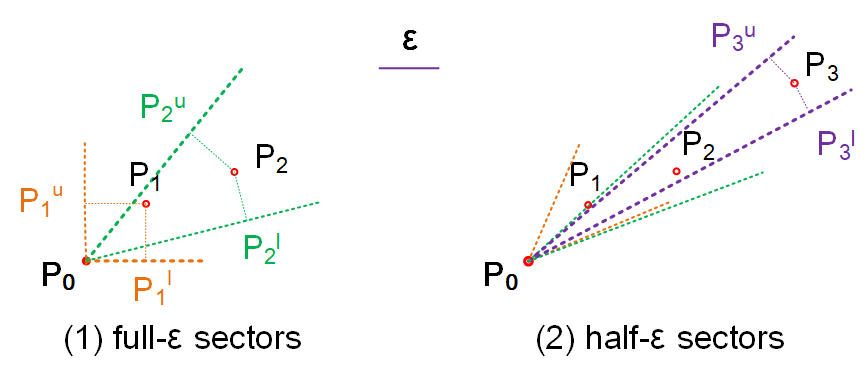
\includegraphics[scale=1.0]{figures/Fig-Sleeve.png}
	\vspace{-2ex}
	\caption{\small Examples of sectors and their intersection.}
	\vspace{-2ex}
	\label{fig:sleeve}
\end{figure}


\subsection{Tracking with cones and sectors}


%\ped is familiar in trajectory simplification, where an error-bounded algorithm using \ped always ensures that the original data points live in strip-like areas built from the simplified trajectory. 
%Though \ped is not seemed in position and trajectory tracking, indeed, the sector built from \ped is applicable to track a moving object in a strip area, like the spatio-temporal cone built from \sed that is used to track trajectory in a circular area.


First, similar as the spatio-temporal cones built from \sed are used in simplifying trajectory in circular areas, a mechanism based on sectors built from \ped is used to simplify trajectory in strip areas. Here, a \emph{sector} is largely a simplified version of a spatio-temporal cone projected on an $x$--$y$ 2D space that the temporal information is ignored, that converts the \ped distance tolerance into an angle tolerance for efficiently checking the successive data points. 
Then \textit{sector intersection} \cite{Williams:Longest, Sklansky:Cone, Dunham:Cone, Zhao:Sleeve}, originally developed in fields of computational geometry and cartography to efficient simplifies the border lines of a geometric or cartographic shape in digital format, is an efficient and effective way to simplify trajectories as pointed out in \cite{Lin:Cised}.
We next demonstrate that it is also applicable to track trajectory in strip areas.


\begin{theorem}
	\label{theo-half-sector}
	Given a sub-trajectory $[P_s,...,P_{s+k}]$ and an error bound $\epsilon$, the trajectory can be tracked in a strip area by an approach based on the intersection of sectors.
\end{theorem}

Because the half-$\epsilon$ sector approach of \cite{Williams:Longest, Sklansky:Cone,Zhao:Sleeve} may limit the performance of compression ratio, we also extend it to full-$\epsilon$ sectors for better performance.

\begin{theorem}
	\label{theo-full-sector}
	Given a sub-trajectory $[P_s,...,P_{s+k}]$ and an error bound $\epsilon$, $ped(P_{s+i}, \overline{P_sP_{s+k}})\le \epsilon$ for each $i \in [1,k]$ if line segment $\overline{P_sP_{s+k}}$ passes through $\bigsqcap_{i=1}^{k-1}$\sector{(P_s, P_{s+i}, \epsilon)} - \{$P_s$\} ~and~ $|P_sP_{s+k}| \ge \sqrt{l_{m}^2 - \epsilon^2}$, where $l_{m} = max\{|P_sP_{s+i}|\}$ for each $i \in (0, k)$.
\end{theorem}

Theorem \ref{theo-full-sector} tells that full-$\epsilon$ sector approach with constrains that (1) $\overline{P_sP_{s+k}}$ lives in the common intersection of the preview full-$\epsilon$ sectors and (2) $|P_sP_{s+k}|$ is longer than $\sqrt{l_{m}^2 -\epsilon^2}$, is applicable to simplify and track a moving object in a strip area. Because the full-$\epsilon$ sector and $|P_sP_{s+k}| \ge \sqrt{l_{m}^2 - \epsilon^2}$ are looser constraints than the half-$\epsilon$ sector and $|P_sP_{s+k}| \ge l_{m}$ used in \cite{Williams:Longest, Sklansky:Cone,Zhao:Sleeve}, this new approach is sure of bringing a better compression ratio.

\eat{%%%%%%%%%%%%%%%%%%%
	\begin{theorem}
		\label{theo-sector-vs}
		Given a sub-trajectory $[P_s,...,P_{s+k}]$ and an error bound $\epsilon$, if $\bigsqcap_{i=1}^{k}$\sector{(P_s, P_{s+i}, \epsilon/2)} $\ne \{P_s\}$, then $\overline{P_sP_{s+k}}$ passes through $\bigsqcap_{i=1}^{k-1}$\sector{(P_s, P_{s+i}, \epsilon)}-$\{P_s\}$; and the opposite is not necessarily true.
	\end{theorem}
	
	
	Theorem \ref{theo-sector-vs} tells that the full-$\epsilon$ sector approach also brings a better effectiveness than the half-$\epsilon$ sector, hence it is the dominant way to develop trajectory simplification/tracking algorithms.
}%%%%%%%%%%%%%%%%%%%%%%%%





%\myblue{Is there an effective and efficient trajectory algorithm implementing \bed that tracks a moving object in a rectangle-like area? Theorem \ref{theo-binary} is the answer to this question.}
Second, by combining cones and sectors, we are able to efficiently track trajectory in rectangle-like areas.

\begin{theorem}
	\label{theo-binary}
	Given a sub-trajectory $[P_s,...,P_{s+k}]$ and two error bounds $\epsilon_{sed}$ and $\epsilon_{ped}$ satisfying $\epsilon_{sed} > \epsilon_{ped}$, it can be tracked in rectangle-like areas by combining sectors and spatio-temporal cones.
\end{theorem}

To track the positions and at the same time simplify the trajectory in a rectangle-like area, it is important to make sure that during the processing of a sub-trajectory $[P_s,...,P_{s+k}]$, there are the same start point $P_s$ and the same velocity $\vec{v}$ for each technique of spatio-temporal cones, sectors, and position tracking of \ped and \sed, such that a strip and a circle \wrt a velocity $\vec{v}$ or a line segment $\overline{P_sP_{s+i}}$, $0<i\le k$, exactly form a rectangle-like area. This is the guideline to develop such a trajectory tracking algorithm. 



%%%%%%%%%%%%%%%%%%%%%%%%%%%%%%%%%%%%%%%%%%%%%%%%%%%%%%%%%%%%%%%%%%%%%%%%%%
% Algorithm: Traj tracking based on section intersection using full sectors.
\begin{figure}[tb!]   
	\begin{center}
		{\small
			\begin{minipage}{3.3in}
				\myhrule
				%\vspace{-1ex}
				\mat{0ex}{
					{\bf Algorithm}~\bitt $(\dddot{\mathcal{T}}[P_0,\ldots,P_n], ~\epsilon_{sed}, m, ~\epsilon_{ped})$\\
					%	\sstab
					\bcc \hspace{1ex}\= $P_s := P_0$; ~~~~$\mathcal{R}^*$ := \kw{getRPolygon}($P_s$, $P_{s+1}$, $\epsilon_{sed}$, $m$, $P_{s+1}.t$); \\
					\icc \hspace{1ex}\= $\mathcal{S}^*$ := \kw{getSector}($P_s$, $P_{s+1}$, $\epsilon_{ped}$); \\
					\icc \hspace{1ex}\= $|\vv{v}|:=\frac{|P_{s}P_{s+1}|}{P_{s+1}.t-P_s.t}$; ~~~~$\vv{v}.\theta:=\overline{P_{s}P_{s+1}}.\theta$;  \\
					\icc \hspace{1ex}\= update ($P_{s}, \vv{v}$); 	\\
					\icc \hspace{1ex}\= $l_{m} := |P_sP_{s+1}|$; ~~~~$i:= 2$;  	\\
					\icc \hspace{1ex}\= while $i \le n$ do \\
					\icc \>\hspace{3ex} if $\overline{P_sP_{i}}$ ~does not pass~ $\mathcal{R}^*~or~\mathcal{S}^*$, or $|P_sP_{i}| < \sqrt{l_{m}^2 - \epsilon^2}$ ~then \\ % // updates velocity and location \\
					\icc \>\hspace{7ex}    $P_s := P_{i-1}$; ~~~~$\mathcal{R}^*$ := $\emptyset$;~~~~$\mathcal{S}^*$ := $\emptyset$; ~~~~$l_{m} := 0$;\\
					\icc \>\hspace{7ex}    $|\vv{v}|:=\frac{|P_sP_{i}|}{P_{i}.t-P_s.t}$; ~~~~$\vv{v}.\theta:=\overline{P_{s}P_{i}}.\theta$;  \\
					\icc \>\hspace{7ex}    update ($P_{s}, \vv{v}$); 	\\
					\icc \>\hspace{3ex} else if $sed(P_i, \vv{v}) \ge \epsilon_{sed}$ ~or~ $ped(P_i, \vv{v}) \ge \epsilon_{ped}$ ~then  \\ %$\overline{P_sP_{i}}$ ~passes ~ $\mathcal{R}^*$ and $\mathcal{S}^*$, $|P_sP_{i}| > l_{m} - \epsilon$ \\ \hspace{9ex} ~and~
					\icc \>\hspace{7ex}    $|\vv{v}|:=\frac{|P_sP_{i}|}{P_{i}.t-P_s.t}$; ~~~~$\vv{v}.\theta:=\overline{P_sP_{i}}.\theta$; \\
					\icc \>\hspace{7ex}    update ($\vv{v}$); \\
					\icc \>\hspace{3ex} if $\mathcal{S}^*=\emptyset$ ~then~ $\mathcal{S}^*:=$ \kw{getSector}($P_s$, $P_{i}$, $\epsilon_{ped}$);\\
					\icc \>\hspace{7ex}     $\mathcal{R}^*:=$ \kw{getRPolygon}($P_s$, $P_{i}$, $\epsilon_{sed}$, $m$, $P_{s+1}.t$); \\
					\icc \>\hspace{3ex} else $\mathcal{S}^*$ := $\mathcal{S}^*\bigsqcap$ \kw{getSector}($P_s$, $P_{i}$, $\epsilon_{ped}$); \\
					\icc \>\hspace{7ex}     $\mathcal{R}^*:=\mathcal{R}^*\bigsqcap$ \kw{getRPolygon}($P_s$, $P_{i}$, $\epsilon_{sed}$, $m$, $P_{s+1}.t$);\\
					\icc \>\hspace{3ex} $l_{m} := \max\{|P_sP_{i}|, l_{m}\}$;  ~~~~$i$ := $i +1$;\\
					\icc \>\hspace{0ex} update ($P_{n}$); 
				}
				\vspace{-2ex}
				\myhrule
			\end{minipage}
		}
	\end{center}
	\vspace{-2ex}
	\caption{\small Trajectory tracking based on sector and cone.}
	\label{alg:bitt}
	\vspace{-1ex}
\end{figure}
%%%%%%%%%%%%%%%%%%%%%%%%%%%%%%%%%%%%%

\subsection{Implementation.}
We now present the algorithm of \underline{B}inary \underline{I}ntersection for \underline{T}rajectory \underline{T}racking (BITT) that tracks moving objects in a rectangle-like area of \bed (see Figure~\ref{alg:bitt}). 
%
\bitt is the double checks of cone intersection and sector intersection for each point for the purpose of trajectory simplification, and the double checks of \sed and \ped distance deviations for position tracking. In addition to that, it uses a uniform velocity $\vv{v}$ for position tracking of both \sed and \ped such that either deviation of \ped or \sed distance will cause an update of velocity $\vv{v}$. 
%
\bitt is a position tracking algorithm as well as a trajectory simplification algorithm, and it ensures that any removed point is located in a rectangle-like area around its expected position \wrt a velocity of position tracking or a line segment connecting two neighboring points of the simplified trajectory. 
%\eg $P_2$ is in the rectangle-like area around its synchronized point $P'_2$ \wrt line segment $\overline{P_0P_4}$
%
\bitt is also the super version of \citt, that is, if $\epsilon_{sed} \le \epsilon_{ped}$, then it falls back to \citt. Similarly, if $\epsilon_{sed} >> \epsilon_{ped}$, then ``$\overline{P_sP_{i}}$ does not pass $\mathcal{R}^*$'' of line 7 and ``$sed(P_i, \vv{v}) \ge \epsilon_{sed}$'' of line 11 are always false, thus \bitt degenerates to \underline{S}ector \underline{I}ntersection for \underline{T}rajectory \underline{T}racking (\sitt in short) that tracks trajectory in strip areas.


\begin{example}
	Figure~\ref{fig:sitt} is a running example of \sitt taking the same input as Figure~\ref{fig:citt}. It uses full-$\epsilon$ sectors, (1) $P_4$ lives in the common intersection of \sector{_{1}}, \sector{_{2}} and \sector{_{3}} and it has a \ped distance larger than $\epsilon$ to $\vec{v_1}$, thus, \sitt updates the velocity from $\vec{v_1}$ to $\vec{v_4}$ and the process goes on, and (2) $P_5$ is outside of the common intersection of the preview sectors, thus, $P_4$ serves as the new start point, and an update is triggered. Finally, \sitt sends three points, $P_0, P_4$ and $P_8$, and three velocities, $\vec{v_1}$, $\vec{v_4}$ and $\vec{v_5}$, to the MOD server. 
\end{example}

\begin{figure}[tb!]
	\centering
	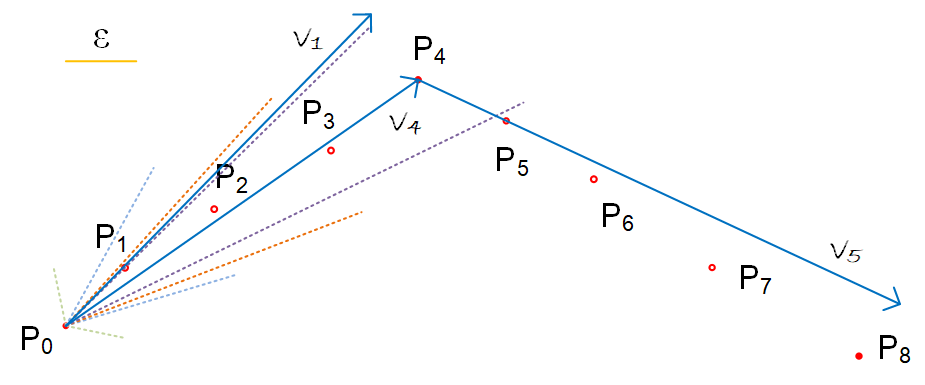
\includegraphics[scale=1.0]{figures/Fig-SITT.png}
	\vspace{-2ex}
	\caption{\small A running example of trajectory tracking by \sitt.  }
	\vspace{-2ex}
	\label{fig:sitt}
\end{figure}



\begin{example}
	Figure~\ref{fig:bitt} is a running example of \bitt. It takes as inputs the same trajectory as the above, the same $\epsilon_{sed}$ as Figure~\ref{fig:citt} and an $\epsilon_{ped}$ of half that of Figure~\ref{fig:sitt}. Because its $\epsilon_{sed}$ is the same as Figure~\ref{fig:citt}, its effectiveness is also the same as Figure~\ref{fig:citt}. For the purpose of clearness, we do not show those cones in the figure.
	%
	\bitt uses full-$\epsilon_{sed}$ cones and full-$\epsilon_{ped}$ sectors to simplify the trajectory. Initially, it sets the same start point and initial velocity as Figure~\ref{fig:citt}, 
	Then, (1) $P_3$ lives in the common intersection of the preview cones and sectors, and it has both \sed and \ped distances larger than $\epsilon_{sed}$ and $\epsilon_{ped}$, respectively, \ie $|P_3P'_3| \ge \epsilon_{sed}$ and $|P_3P^*_3| \ge \epsilon_{ped}$, thus, \bitt updates the velocity from $\vec{v_1}$ to $\vec{v_3}$ and the process goes on, (2) $P_5$ is outside of the common intersections of the preview cones and sectors, thus, $P_4$ serves as the new start point, and an update of $(P_4, \vec{v_5})$ is triggered, and (3) $P_7$ lives in the common intersections of the preview cones and sectors, and it has a \ped distance larger than $\epsilon_{ped}$, thus, \bitt updates the velocity from $\vec{v_5}$ to $\vec{v_7}$ (not shown) and the process goes on. Finally, it sends three points, $P_0, P_4$ and $P_8$, and four velocities, $\vec{v_1}$, $\vec{v_3}$, $\vec{v_5}$ and $\vec{v_7}$, to the MOD server. 
\end{example}

\begin{figure}[tb!]
	\centering
	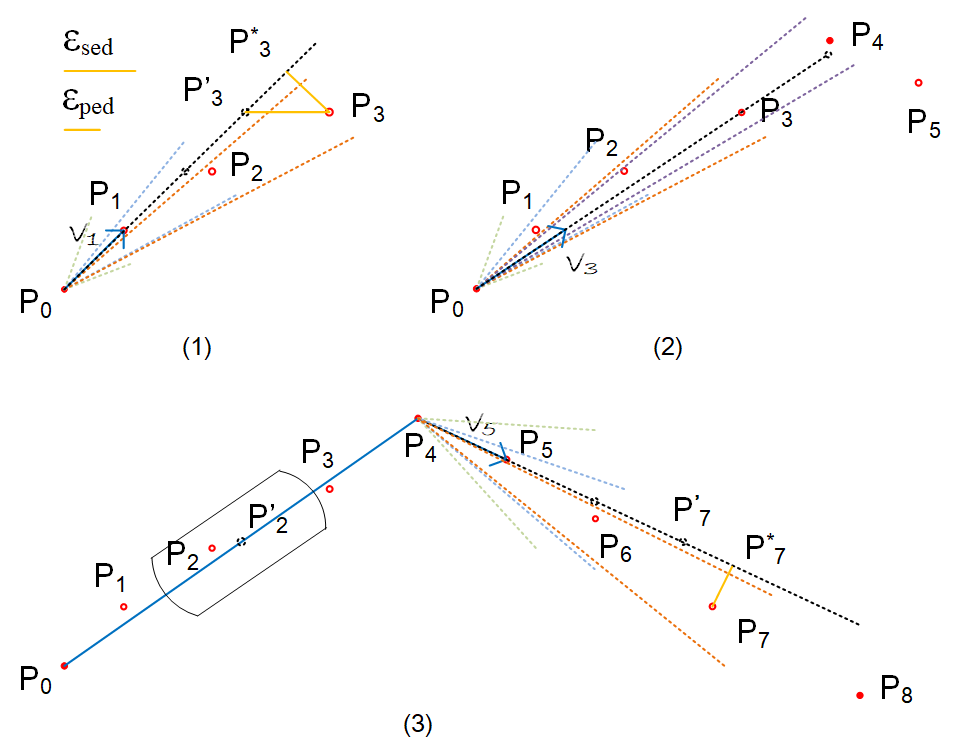
\includegraphics[scale=1.0]{figures/Fig-BITT.png}
	\vspace{-2ex}
	\caption{\small A running example of trajectory tracking by \bitt. In this case, the spatio-temporal cones and their intersections are the same as Figure~\ref{fig:citt}, thus they are not shown here for clearness.  }
	\vspace{-2ex}
	\label{fig:bitt}
\end{figure}





\stitle{Correctness and complexity.} 
\myblue{The correctness of algorithm \bitt follows from Theorems \ref{theo-full-cone}, \ref{theo-full-sector} and \ref{theo-binary}.
It is also easy to find that it has a linear time complexity like \citt and \sitt.}


%\stitle{Discuss.} Relations to position tracking and traj simplification. 
